\section{Füllstruktur am Elektronenspeicherring DELTA}
\label{sec:Einleitung}
Der Dortmunder Elektronenspeicherring DELTA (Dortmund Electron Accelerator) ist eine 
$\SI{1,5}{\giga\electronvolt}$ Synchrotronstrahlungsquelle mit einem Umfang von $\SI{115,2}{\meter}$.
Die bereitgestellte Synchrotronstrahlung wird von verschiedenen Arbeitsgruppen aus den Gebieten der 
Physik, Chemie und Materialwissenschafen genutzt, um meist kondensierte Materie zu untersuchen. Zudem 
wird bei DELTA in immer größerem Maß Grundlagenforschung im Bereich der Beschleunigerphysik betrieben.
Dazu zählen vorallem Konzepte zur erzeugung von ultrakurzen Strahlungspulsen mittels Interaktion von
geladnenen Teilchen, welche sich in periodischen Magnetfeldstrukturen bewegen, mit Laserpulsen 
unterschiedlichster Wellenlängen. Synchrotronstrahlung ist diejenige breitspektrale Strahlung welche 
entsteht wenn, mit elektrischer Ladung belegte Teilchen, beschleunigt werden. In einem Speicherring 
bleiben die geladenen Teilchen zwar in sehr guter Näherung bei gleicher Geschwindigkeit, welche hier 
nahezu die Vakuumlichtgeschwindigkeit ist, jedoch stellt auch ein Richtungswechsel im Laborsystem eine 
Beschleunigung dar, sodas in jeder Kurve des Speicherrings Synchrotronstrahlung abgegeben wird. Die 
Richtungsänderung zur Erhaltung der null-förmigen Sollbahn wird bei DELTA durch elektrische Dipolmagneten, 
welche mit einem Betriebsstrom von etwa $\SI{1}{\kilo\ampere}$ eine magnetische Flussdichte von circa 
$\SI{1,5}{\tesla}$ in der Strahlbahn erzeugen, bewirkt. Die so erzeugte Strahlung nennt sich nach ihrer 
entstehung Dipolstrahlung und kann an 12 Beamlines genutzt werden. Die mit der Strahlung 
ausgekoppelte Energie geht für die umlaufenden Teilchen verloren und muss in als Cavity bezeichneten 
elektromagnetischen Hohlraumresonatoren nachgefüttert werden. Die Cavitys werden mit einer Frequenz von 
knapp $\SI{500}{\mega\hertz}$ betrieben. In den hier beschriebenen Experimenten wird jedoch keine 
Dipolstrahlung verwendet sondern Undulatorstrahlung. Diese entsteht wenn ein geladenes Teilchen eine 
Anordnung von abwechselnd gepolten Magneten durchläuft. Diese Abfolge wird Undulator genannt. Die 
entstehende Strahlung ist im Spektrum wesentlich schmaler als die Dipolstrahlung am selben Speicherring.
Bei DELTA werden zur Strahlungserzeugung Elektronen verwendet. Diese sind besonders geeignet da sie sich
aufgrund ihrer geringen Ruhemasse leicht beschleunigen und ablenken lassen. Eine wichtige 
characteristische Größe eines Speicherrings für geladenen Teilchen ist der maximale Strahlstrom. Dieser 
ist definiert als Zahl der Ladungen die pro Zeiteineheit eine Fläche durchqueren.
Der maximale Strahlstrom im Multibunchbetrieb liegt am DELTA bei etwa $\SI{130}{\milli\ampere}$.
Der Elektonenstrahl ist an dieser Maschine in 192 Buckets mit einer Länge von etwa $\SI{0,6}{\meter}$, 
was bei Lichtgeschwindigkeit etwa $\SI{2}{\nano\second}$ entspricht, aufgeteilt. In jedem Bucket können 
sich unterschiedlich viele Elektronen befinden. Ein Bucket bezeichnet hier eine Art räumlichen Abschnitts 
im mitbewegten Bezugssystem. Die Gruppe von Elektronen die sich in jedem Bucket befinden kann, besitzt 
bei Lichtgeschwindigeit eine Länge von etwa $\SI{36}{\pico\second}$ und wird als Bunch bezeichnet. Die 
Kombination von unterschiedlich stark gefüllten Buckets wird Füllstruktur genannt. DELTA kann mit drei 
verschiedenen Typen von Füllstrukturen betrieben werden.

\subsection{Singlebunch}
\label{sec:Singlebunch}
Im Singlebunchbetrieb wird nur ein einzelner Bucket mit einem einzelnen Bunch befüllt. Das hat zur Folge
das mit einer Frquenz von etwa $\SI{2,6}{\mega\hertz}$ etwa alle $\SI{384}{\nano\second}$ ein kurzer 
Strahlungsblitz erzeugt wird. Eine Variante dieses Betriebsmodus ist der Betrieb mit einem einzelnen
Elektron. Dazu wird im Singlebunchbetrieb ein Bucket mit einer geringen Zahl Elektronen befüllt. Im 
nächsten Schritt wird dann eine art Stempel, Scraper genannt, nah an den Elektronenstrahl herngefahren.
Da die Elektronen sich nun nicht, wie an einer Perlenkette aufgereiht präzise auf ihrer Sollbahn fliegen,
sondern vielmehr transversal um diese Sollbahn schwingen, treffen immer wieder Elektronen auf den Scraper
und gehen somit für den eigentlichen Strahl verloren. Die Ausdehnung des Strahls verringert sich durch den 
Verlust der stark schwingenden Elektronen. Der Scraper wird nun Schritt für Schritt näher an den Strahl 
herangefahren bis nurnoch ein einzelnes Elektron übrig ist.

\subsection{Multibunch}
\label{Multibunch}
Der Multibunchbetrieb stellt die Standardfüllstruktur bei DELTA dar. Hier werden 128 der Buckets mit 
einer ähnlichen Anzahl von Elektronen befüllt, darauf folgen dann 64 ungefüllte Buckets. Das bedeutet es 
wird eine Abfolge von 128 kurzen Strahlungsblitzen mit einem Absand von jeweils etwa 
$\SI{2}{\nano\second}$ erzeugt auf welche eine Strahlungsfreie Periode von etwa $\SI{128}{\nano\second}$
folgt.

\begin{figure}
    \centering
    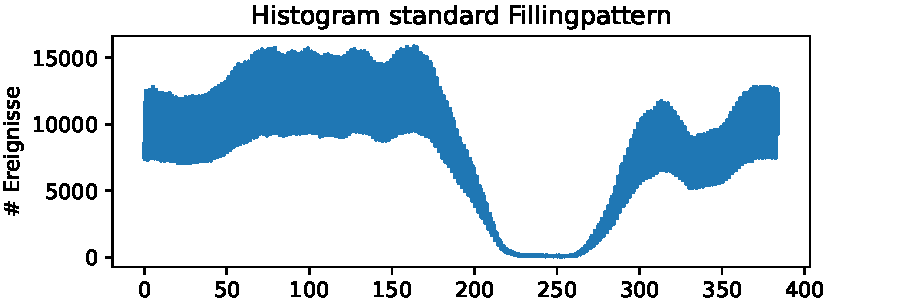
\includegraphics{content/plots/standardfillingpattern.pdf}
    \caption{nix}
    \label{fig:standardfillingpattern}
  \end{figure}


\subsection{Hybride Füllstruktur}
\label{sec:HybrideFuellstruktur}
Die hybride Füllstruktur zeichnet sich dadurch aus das der Speicherring zunächst im Multibunchbetrieb
gestartet wird und dann in ein Bucket das zur strahlungsfreien Periode gehört Elektronen injiziert werden.

\begin{figure}
    \centering
    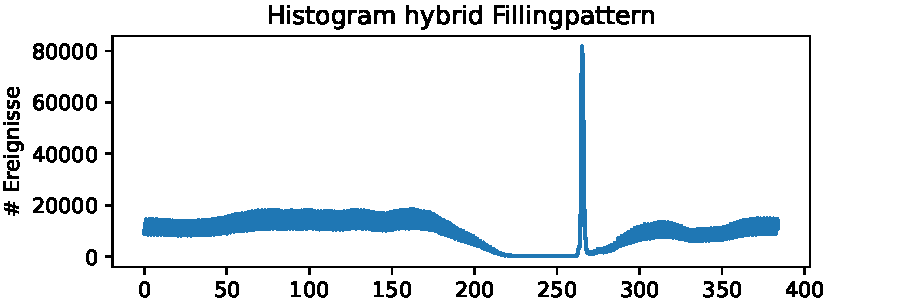
\includegraphics{content/plots/hybrid.pdf}
    \caption{nix }
    \label{fig:hybridfillingpattern}
  \end{figure}

\subsection{Bisherige Messung der Füllstruktur}
\label{sec:WasBisherGeschah}
Bisher wird die Füllstruktur gemessen indem das Signal eines BPMs (Beam Position Monitors) mit einer
Oszilloskopkarte ausgewertet wird. Ein solcher BPM besteht aus vier sogenannter Pickupelektroden
welche in der zum Strahl transversalen Ebene in die Bahn eingebracht wurden. Wenn nun ein Elektronenpaket
diese Ebene quert, erzeugt es in den Elektroden Spiegelladungen, daher kann eine kleine Spannung gemessen 
werden. Aus den vier Spannungen kann dann die transversale Strahllage berechnet werden. Um die Füllstruktur
zu errechnen müssen jedoch alle vier Spannungen in einem Leistungsaddierer addiert werden. Dabei gilt:
je größer das Gesamtsignal desto größer die Ladungsmenge im Bunch. Das entstehende 
Summensignal wird an eine Oszilloskopkarte weitergeleitet dort aufgezeichnet, verarbeitet und über das 
EPICS (Experimental Physics and Industrial Control System) an den Kontrollraum weitergeleitet wo es
als Balkendiagram mit der Bucketnummer auf der Abszisse und der Ladungsmenge auf der Ordinate dargestellt 
wird.



